\documentclass{report}

% Language packages
\usepackage[utf8]{inputenc}
\usepackage[T1]{fontenc}
\usepackage[portuguese]{babel}

% Code related packages/commands
\usepackage{caption}
\usepackage[newfloat]{minted}

\usepackage{hyperref}


\newcommand{\todo}[1]{{\color{red} #1}}

\title{AMD Memory Encryption: SME e SEV}

\author{João Gabriel Trombeta\\
        João Paulo Taylor Ienczak Zanette\\
        Ranieri Schroeder Althoff}
\date{\today}

\begin{document}

\maketitle

\tableofcontents

\chapter{Máquinas Virtuais}

Máquinas virtuais (VM, na sigla em inglês para \textit{Virtual Machines}) são
emuladores de computadores lógicos, implementando arquiteturas e conjuntos de
instruções para prover a funcionalidade de um computador físico. Chama-se de
\textit{Guest} ou convidado o computador executado pela máquina virtual, e de
\textit{Host} ou hospedeiro o computador cujo \textit{hardware} oferece
recursos para executar a máquina virtual. No \textit{Host}, uma camada de
software chamada hypervisor permite a execução máquinas virtuais em uma máquina
física, independentes entre si e executando sistemas operacionais semelhantes
ou não.

\section{Hypervisor}

Também chamado de monitor de máquina virtual (VMM, na sigla em inglês para
\textit{Virtual Machine Monitor}), um \textit{hypervisor} é um componente em
forma de \textit{hardware}, \textit{software} ou \textit{firmware}, responsável
por criar e executar uma máquina virtual. \textit{Hypervisors} podem ser do
tipo nativo (ou \textit{bare metal}), quando executa suas máquinas virtuais
diretamente no \textit{hardware} do \textit{Host}, ou \textit{Hosted}, quando
executa \textit{software} sobre o sistema operacional do \textit{Host}, sendo
gerenciado pelo \textit{kernel} do mesmo.

O \textit{hypervisor} é responsável pela camada de abstração entre o
\textit{Host} e os \textit{Guests}, realizando o gerenciamento de recursos,
pois um \textit{Guest} individualmente é isolado de forma que todos os recursos
de \textit{hardware} visíveis são considerados seus. Cada máquina virtual deve
ser gerenciada de forma a evitar que comprometa o funcionamento das outras, por
isso toda interação com o meio físico é intermediada pelo \textit{hypervisor},
que é fortemente protegido das máquinas virtuais por ele gerenciadas.

\section{Falhas em Hypervisors}

\subsection{Xen Hypervisor}

Uma falha de segurança detectada com relação a \textit{hypervisors} foi
explorada no \textbf{Xen Hypervisor}, um dos \textit{hypervisors} mais
populares da atualidade, em que é possível executar uma função arbitrária
alterando a tabela de \textit{hypercalls}, algo semelhante a uma
\textit{vtable} no contexto de \textit{hypervisors}. Uma \textit{hypercall} é
uma \textit{software trap} (uma interrupção) do \textit{hypervisor} para
executar operações privilegiadas, como atualizar tabelas de página das máquinas
virtuais.

Para explorar a falha, primeiramente é necessário descobrir a localização da
tabela de \textit{hypercalls} procurando pela assinatura da página, que é dada
pelo \textit{checksum} de seu conteúdo. Como a página não possui um formato tão
previsível, é difícil de localizá-la, mas a tabela de argumentos dos
\textit{hypercalls} possui um formato previsível, já que seu conteúdo, que é o
número de argumentos de cada \textit{hypercall}, é fixo, e portanto seu
\textit{checksum} também é previsível. Além disso, a tabela de argumentos
sempre se encontra na página seguinte à tabela de \textit{hypercalls}, o que
implica que basta encontrar uma das tabelas para que se tenha a localização da
outra.

Aliado à possibilidade de leitura e escrita de código arbitrário, feito através
de falhas nas regras de verificação de segurança de escrita em páginas do
\textit{hypervisor}, é possível então efetuar escape de máquina virtual, por
exemplo, acessando recursos do \textit{Host} que não estão alocados para
máquina virtual.

\chapter{AMD Memory Encryption}

A AMD possui dois mecanismos de encriptação de memória com a finalidade de
tornar mais seguro o uso de máquinas virtuais, são o Secure Memory Encryption
(SME) e Secure Encrypted Virtualization (SEV). Para realizar tal função, ambos
utilizam o AMD Secure Processor.

\section{AMD Secure Processor}

Grande parte das funções de criptografia executadas em um processador AMD
utilizam um processador dedicado e independente, o \textbf{AMD Secure
Processor} (AMD-SP, chamado anteriormente de \textbf{Platform Security
Processor}), que garante que componentes sensíveis à segurança não recebam
interferência do \textit{software} sendo executado nos processadores
principais.

O AMD-SP roda um \textit{kernel} seguro de código fechado, que pode executar
tarefas do sistema assim como tarefas de terceiros confiáveis, tendo o
administrador controle sobre quais tarefas de terceiros são designadas ao
processador. Além disso, possui uma memória dedicada e acesso direto ao
coprocessador criptográfico (CCP), que é composto por um gerador de números
aleatórios, várias engines para o processamento de algoritmos de criptografia,
e um bloco para o armazenamento de chaves.

\section{Security Memory Encryption}

O \textbf{AMD Secure Memory Encryption} (SME) é um mecanismo que pode ser
utilizado para criptografar os dados que são escritos na RAM, com a finalidade
de evitar ataques físicos. Durante o boot, o AMD-SP gera uma chave simétrica
que será usada para criptografar e descriptografar os dados que transitam pela
DRAM\@. Como a \textit{engine} de criptografia está dentro do chip, o impacto
das operações é pequeno.

\begin{figure}[h]
    \centering
    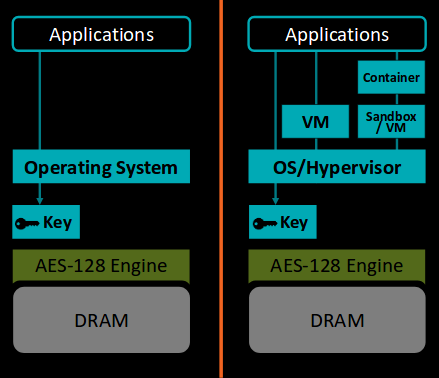
\includegraphics[width=0.5\textwidth]{img/sme}
    \caption{Método de criptografia do SME}\label{sme-1}
\end{figure}

A figura~\ref{sme-1} mostra como ocorre a criptografia. A \textit{engine} é
localizada entre o sistema operacional ou \textit{hypervisor} e a memória, onde
a informação é criptografada utilizando a chave indicada antes de ser salvo na
DRAM. Ao ser posteriormente carregado da DRAM para o sistema operacional
novamente, as informações são descriptografadas.

Este mecanismo de segurança não previne ataques provenientes de um
\textit{hypervisor} nativo comprometido, uma vez que ele possui acesso aos
dados de maneira direta, sem criptografia. O objetivo, então, é de evitar
ataques do tipo \textit{probe attack} na memória, instalação de
\textit{hardware} que possa acessar a memória do \textit{guest} em texto plano,
ou ataques que possam capturar dados de DIMM e NVDIMM.

Para utilizar o SME, é necessário verificar se o processador possui suporte
para este recurso, através da chamada de CPUID Fn8000\_001F, e que durante o
boot, o bit 23 de SYSCFG MSR esteja ativado para sinalizar que esse recurso
está habilitado. Após a verificação, ao realizar acesso à DRAM, o bit mais
significativo do endereço, chamado de C-bit, sinaliza se o dado deve ou não ser
criptografado.

\begin{figure}[h]
    \centering
    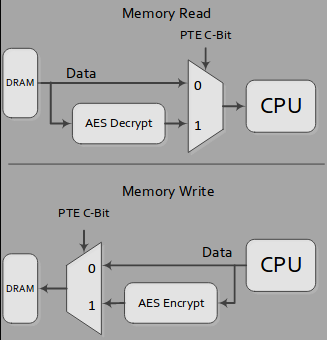
\includegraphics[width=0.5\textwidth]{img/sme_read_write_architecture.png}
    \caption{Leitura e escrita no SME}\label{sme-read-write}
\end{figure}

Como visto na figura~\ref{sme-read-write}, para a leitura da memória, antes do
dado ser copiado para a CPU, duas versões do dado são inseridas como entrada de
um multiplexador, uma com o dado literal como estava na DRAM, outra com o dado
descriptografado, após passar pelo circuito responsável. O controle do
multiplexador recebe o bit mais significativo do endereço, o C-bit, para
selecionar entre as entradas caso o dado esteja na região criptografada ou não.
Para a escrita, a ideia é semelhante e inversa, selecionando entre o dado
criptografado ou literal.

Existe uma variação chamada \textbf{Transparent SME}, onde tudo é
criptografado. Neste caso, não é necessário suporte do sistema operacional,
tendo em vista que não é preciso fazer o controle de quais endereços serão
criptografados e quais não serão. O processo de acesso à memória ocorre da
mesma forma que no SME.


\section{Secure Encrypted Virtualization}

\textbf{Secure Encrypted Virtualization} (SEV) integra o SME com a capacidade
de comportar várias VMs criptografadas. Durante o boot, a máquina \textit{host}
recebe uma chave, a qual é utilizada da mesma maneira que em SME. O diferencial
do SEV é que, após a inicialização, cada máquina virtual também ganha uma chave
única, podendo assim criptografar seus dados e protegê-los, tanto do
\textit{hypervisor} como de outros \textit{guests} sendo executados no
\textit{host}.

\begin{figure}[h]
    \centering
    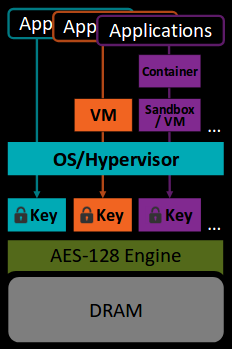
\includegraphics[width=0.5\textwidth]{img/sev}
    \caption{Demonstração do acesso à memória através de chaves.}\label{sev}
\end{figure}

A figura~\ref{sev}, apesar de muito similar a~\ref{sme-1}, mostra como o acesso
à memória se dá com a utilização sempre da chave correspondente à máquina que
realizou a operação.


\begin{figure}[h]
    \centering
    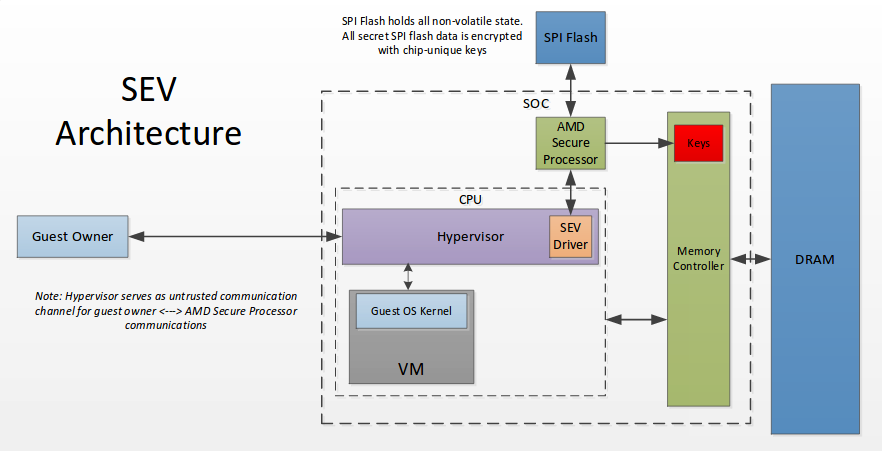
\includegraphics[width=1\textwidth]{img/sev-architecture}
    \caption{Visão geral da arquitetura do SEV\@.}\label{sev-architecture}
\end{figure}

Na figura~\ref{sev-architecture} é demonstrada a visão geral da arquitetura do
SEV, nela é possível encontrar:

\begin{description}
    \item[Guest Owner]: Usuário que contratou o serviço e interage com sua VM\@.
    \item[Hypervisor]: Interage com as VMs e com o Secure Processor através de
    drivers.
    \item[VM]: Virtual Machine sendo executada no \textit{Host}.
    \item[Secure Processor]: Tem acesso exclusivo ao banco de chaves e interage
    com o SPI flash.
    \item[SPI Flash]: Utilizado para o gerenciamento de chaves.
    \item[Memory Controller]: Controla os acessos à memória aplicando
    conceitos visto acima, como por exemplo a criptografia.
    \item[DRAM]: Memória que armazena os dados dos \textit{Guest}s e do \textit{Host}.
\end{description}

\begin{figure}[h]
    \centering
    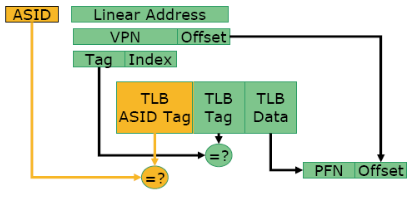
\includegraphics[width=0.5\textwidth]{img/asid}
    \caption{Comportamento da TLB mediante ASID\@.}\label{asid}
\end{figure}

Para implementar essa tecnologia também é usado o Address Space ID (ASID) para
identificar a chave que pertence à VM\@. Para tirar proveito disso, o
identificador também é utilizado para definir de quem é um dado na TLB, assim a
ASID também é usado como uma \textit{tag} na TLB\@. Após uma tentativa de
acessar o dado, depois de ser encontrado pela TLB, é feita uma verificação para
garantir que os identificadores são correspondentes antes de garantir um TLB
hit. Isso faz com que não seja necessário esvaziar a TLB em caso de troca de
contexto entre VMs, uma vez que as \textit{tags} não irão colidir com uma mesma
região da TLB\@. Esse comportamento é demonstrado em~\ref{asid}.

\begin{figure}[h]
    \centering
    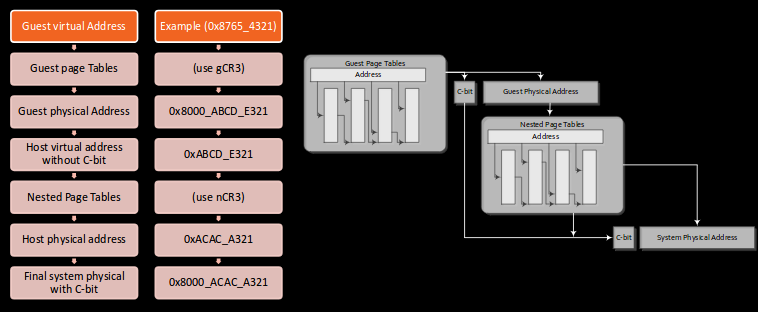
\includegraphics[width=1\textwidth]{img/sev-address-translation}
    \caption{Tradução de endereços do SEV\@.}\label{sev-address-translation}
\end{figure}

Um exemplo da tradução de endereço é visto em~\ref{sev-address-translation}.
Primeiramente o \textit{Guest} traduz o endereço para o que ele acredita ser o
endereço físico. Após isso o \textit{Host} calcula o real endereço físico
requisitado, deixando de lado o C-bit. Uma vez que o endereço físico é
encontrado, o C-bit é novamente inserido e o dado pode ser consultado na
memória.

Além disso, é possível existir conflito ao decidir se uma página é
criptografada ou não. Uma página do \textit{Guest} pode ter o C-bit marcado
como 0, mas sua página física correspondente no \textit{Host} ter C-bit 1.
Nesses caso a página seria criptografada com a chave do \textit{Host}, porém
caso os dois C-bits sejam 1 o \textit{Guest} teria prioridade, logo a chave
usada seria a sua.

O SEV poderia garantir proteção contra o exploit visto em 1.3.1. Uma tentativa
de analisar o \textit{checksum} com páginas criptografadas seria um desafio
muito maior, já que o passo base do \textit{exploit} consiste no \textit{Guest}
varrer dados do \textit{Host}. Com a criptografia de memória, o \textit{Guest}
acabará descriptografando os dados do \textit{Host} usando a própria chave,
obtendo respostas diferentes do esperado e portanto não conseguindo identificar
a tabela de argumentos de \textit{Hypercall}. Caso a VM ainda assim conseguisse
controle do \textit{Host}, outras VMs estariam protegidas por utilizar sua
própria chave. No geral o SEV consegue lidar tanto com ataques físicos quanto
ataques de usuário, como o \textit{Host} injetar código nos \textit{Guest}s ou
algum \textit{Guest} tomar controle do \textit{Host}.

\section{Utilização do SME e SEV}

\subsection{\textit{Set-up} e comunicação}

\begin{table}[h]
    \centering
    \begin{tabular}{lll}
        \toprule
        Status  & Código\\
        \midrule
        SUCCESS & 0000h\\
        INVALID\_PLATFORM\_STATE & 0001h\\
        INVALID\_GUEST\_STATE & 0002h\\
        INVALID\_CONFIG & 0003h\\
        INVALID\_LENGTH & 0004h\\
        ALREADY\_OWNED & 0005h\\
        INVALID\_CERTIFICATE & 0006h\\
        POLICY\_FAILURE & 0007h\\
        INACTIVE & 0008h\\
        INVALID\_ADDRESS & 0009h\\
        BAD\_SIGNATURE & 000Ah\\
        BAD\_MEASUREMENT & 000Bh\\
        ASID\_OWNED & 000Ch\\
        INVALID\_ASID & 000Dh\\
        WBINVD\_REQUIRED & 000Eh\\
        DFFLUSH\_REQUIRED & 0009h\\
        INVALID\_GUEST & 0010h\\
        INVALID\_COMMAND & 0011h\\
        ACTIVE & 0012h\\
        HWERROR\_PLATFORM & 0013h\\
        HWERROR\_UNSAFE & 0014h\\
        UNSUPPORTED & 0015h\\
        INVALID\_PARAM & 0016h\\
        \bottomrule
    \end{tabular}
    \caption{Relação dos códigos de status dados pelo AMD-SP\@. Mais detalhes
             sobre a tabela estão
             em~\cite{sev-api-doc}}\label{cmdresp-status-code}
\end{table}



A comunicação entre o AMD-SP e o x86 se dá por meio de registradores MMIO
(\textit{Memory Mapped IO}), chamados de \textit{``mailbox registers''}. Um
\textit{mailbox} essencial é o \textit{``Command buffer''}, que será
lido/escrito pelo \textit{Driver} responsável pela implementação do SEV para
enviar comandos relacionados ao SEV para o \textit{firmware}. Primeiramente é
necessário, além de alterar o MSR, definir o endereço de memória em que ficará
o \textit{Command Buffer}, separado em dois registradores:
\texttt{CmdBufAddr\_Hi} e \texttt{CmdBufAddr\_Lo} (32 bits mais e menos
significativos, respectivamente).  Internamente, o registrador do
\textit{Command Buffer} é chamado de \texttt{CmdResp}, e é utilizado da forma:

\begin{enumerate}
    \item O driver (em x86) altera o \texttt{CmdResp} com:
        \begin{itemize}
            \item Bit 31 em 0 (simbolizando a emissão de um comando);
            \item Bits 30 a 26 mantidos em 0 (pois são reservados);
            \item Bits 25 a 16 com o ID do comando a ser emitido;
            \item Bits 15 a 1 também são mantidos em 0 (por serem reservados);
            \item Bit 0 pode ser colocado em 1 para informar o
                \textit{firmware} para habilitar uma interrupção no x86 ao
                completar o comando, do contrário pode ser mantido em 0.
        \end{itemize}
    \item O AMD-SP executa o comando;
    \item Após completar o comando, o AMD-SP escreve no \texttt{CmdResp} com o
        resultado da execução do comando, da forma:
        \begin{itemize}
            \item Bit 31 em 1 para indicar que se trata de uma resposta;
            \item Bits 15 a 0 com o código de status descritos na
                tabela~\ref{cmdresp-status-code}.
        \end{itemize}
\end{enumerate}

\subsection{Comandos}

\subsubsection{INIT}

O comando \texttt{INIT}, intuitivamente, inicializa a plataforma. Isso é feito
carregando os dados de persistência relacionados ao SEV, vindos de algum
armazenamento não-volátil, e inicializando o contexto da plataforma.
Geralmente, os casos em que este não é o primeiro comando executado são os que
primeiramente utilizam comandos como \texttt{PLATFORM\_STATUS} para determinar
a versão da API\@. Requer que o estado da plataforma seja
\texttt{PSTATE.UNINIT};

\subsubsection{SHUTDOWN}

Utilizado pelo dono da plataforma afim de alterar o estado dela para
não-inicializado. A plataforma pode estar em qualquer estado e, quando
executado, todo o estado da plataforma e dos \textit{Guests} é excluído do
armazenamento volátil.

\subsubsection{PLATFORM\_RESET}

Reinicia os dados não-voláteis de SEV, sendo útil quando o dono deseja
transferir a plataforma para um novo dono ou apenas liberar os recursos do
sistema seguramente.

\subsubsection{PLATFORM\_STATUS}

Informa sobre o status atual da plataforma, incluindo versão da API
(\textit{major} e \textit{minor}), dono (se é o próprio \textit{Host} ou é
externo), ID da \textit{build} do \textit{firmware}, número de \textit{Guests}
válidos mantidos pelo \textit{firmware}, e código de status do
\textit{firmware}.

\subsubsection{Outros comandos}

Há outros comandos relativos às chaves, como \texttt{PEK\_GEN},
\texttt{PEK\_CSR}, \texttt{PEK\_CERT\_IMPORT}, \texttt{PDH\_GEN} e
\texttt{PDH\_CERT\_EXPORT}, que permitem gerar, trocar e validar chaves.

\section{Possíveis falhas}

Apesar das seguranças em criptografia os dois sistemas ainda podem ser
vulneráveis a ataques. Nada impede um Hypervisor comprometido de modificar
trechos de um \textit{Guest}, mesmo que por textos sem sentido, ou até mesmo
reescrever dados em um local da memória com trechos mais antigos do mesmo
local.

Outra técnica de ataque que pode ser utilizada pelo Hypervisor é trocar os
dados de dois endereços de uma virtual machine. Dessa forma a VM ainda
conseguiria descriptografar a página porém resultaria em um comportamento
inesperado.

\bibliographystyle{ieeetr}
\nocite{*}
\bibliography{references}

\end{document}
